\documentclass[11pt,xcolor=svgnames]{beamer}
\usepackage{dsfont,natbib,setspace,changepage,multirow,times}
\mode<presentation>

% replaces beamer foot with simple page number
\setbeamertemplate{navigation symbols}{}
\setbeamercolor{frametitle}{fg=black}
\newcommand{\theme}{\color{Maroon}}

\setbeamertemplate{footline}{
   \raisebox{5pt}{\makebox[\paperwidth]{\hfill\makebox[20pt]{\color{gray}\scriptsize\insertframenumber}}}}

\usepackage{tikz}
  
\graphicspath{{/green/Dropbox/inputs/},
{/Users/mtaddy/Dropbox/inputs/},
{/home/taddy/teaching/datamining/graphs/},
{/Users/mtaddy/teaching/datamining/graphs/},
{/Users/mtaddy/datamining/graphs/}}

\setbeamercolor{whitebox}{bg=gray!10}

% colors
\newcommand{\bk}{\color{black}}
\newcommand{\rd}{\color{red}}
\newcommand{\fg}{\color{ForestGreen}}
\newcommand{\bl}{\color{blue}}
\newcommand{\gr}{\color{black!60}}
\newcommand{\sg}{\color{DarkSlateGray}}
\newcommand{\br}{\color{SaddleBrown}}
\newcommand{\nv}{\color{Navy}}


% common math markups
\newcommand{\bs}[1]{\boldsymbol{#1}}
\newcommand{\mc}[1]{\mathcal{#1}}
\newcommand{\mr}[1]{\mathrm{#1}}
\newcommand{\bm}[1]{\mathbf{#1}}
\newcommand{\ds}[1]{\mathds{#1}}
\newcommand{\indep}{\perp\!\!\!\perp}

% spacing and style shorthand
\setstretch{1.1}

% shorthand
\newcommand{\sk}{\vspace{.5cm}}
\newcommand{\R}[1]{{\tt \nv #1}}
\newcommand{\til}{{\footnotesize$\bs{\stackrel{\sim}{}}$}}
\DeclareSymbolFont{extraup}{U}{zavm}{m}{n}
\DeclareMathSymbol{\vardiamond}{\mathalpha}{extraup}{87}


\begin{document}

\setcounter{page}{0}
{ \usebackgroundtemplate{\includegraphics[height=\paperheight]{/Users/mtaddy/Dropbox/inputs/phoenix}}
\begin{frame}[plain]
\begin{center}


{\bf \Huge \theme The Gamma Lasso }

\vskip 1cm
Matt Taddy, University of Chicago Booth School of Business

\vskip .2cm
\texttt{faculty.chicagobooth.edu/matt.taddy/research}

\end{center}
\end{frame} }

\begin{frame}
{penalized deviance estimation}


Estimate regression coefficients for $\bm{y} \approx f(\bm{X}\bs{\beta})$ by solving
{\Large\vspace{-.25cm}\[\nv
{\tt min}\{~l({\bs{\beta}}) + \lambda c(\bs{\beta})~\}.\]}
$\bullet$ $l(\bs{\beta})$ is [proportional to] a negative log likelihood, like SS $0.5\sum_i \left(y_i - \bm{x}_i'\bs{\beta}\right)^2$ or logistic  loss $\sum_i \left[
\log(1+e^{\bm{x}_i'\bs{\beta}})-\bm{x}_i'\bs{\beta}y_i \right]$.  

\vskip .25cm
$\bullet$ $c(\bs{\beta})$ is a positive cost function, often $\|\bs{\beta}\|_q$.

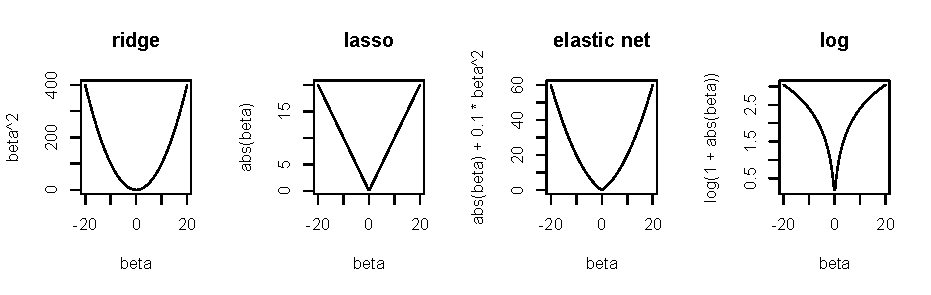
\includegraphics[width=4.25in]{../graphs/penalties}

{\theme Today, we'll talk about costs that behave as if $q \in [0,1]$.}

\vspace{-.25cm}
\end{frame}

\begin{frame}
{regularization paths}

\sk
Since we don't know $\lambda$, the penalization doesn't actually {\it do} model selection.  Instead, it {\it indexes} a set of candidate models.

\vskip .1cm
{\gr Think of $\lambda$ as a signal-to-noise filter: like squelch on a radio.}

\sk
Fortunately, path algorithms can do fast fits over grids of $\lambda_t$:
\begin{itemize}
\item Start at $\lambda_1$ large enough that $\bs{\hat\beta}^1 = \bm{0}$.
\item Incrementally decrease $\lambda_t = \delta \lambda_{t-1}$, $\delta \in (0,1)$.
\item Re-fit coefficients $\bs{\hat\beta}^t$, using $\bs{\hat\beta}^{t-1}$ as hot-starts.
\end{itemize}
{\it If} the coefficients change little under small changes to $\lambda$, \\then a full path can take far less time then a single OLS fit.

\vskip .25cm
{\gr The `if' here is stability: continuity of the regularization path.}

\end{frame}

\begin{frame}
{big data why?}

\vskip .25cm
Consider massive $n\times D$ count matrices $\bm{Y}$, \\paired with an $n\times K$ attribute matrix $\bm{X}$. 


\vskip .25cm
{\nv Congressional Speech }
\vskip .1cm
{\footnotesize
\begin{tabular}{|c|c|c|c|c|c|c}
Name & Congress & State & Party &  Death Tax & Estate Tax & $\cdots$
\\ \hline
T. Cruz & 113 & TX & {\sf gop}  & 18 &
  0 &  \\ 
C. Schumer & 113 & NY & {\sf dem}  & 1 &
  8 & 
\end{tabular}}

\hskip 5cm $\ddots$


{\nv Web Analysis }
\vskip .1cm
{\footnotesize
\begin{tabular}{|c|c|c|c|c|c}
User ID & Age & Purchases &  Motors VIPV & Jewlery VIPV 
& $\cdots$ \\ \hline
JK101 & 33 & \$99.99  &   54 & 10 & 
\end{tabular}}

\hskip 5cm $\ddots$

\vskip .1cm
The dataset is both wide (big $p = D+K$) and long (big $n$).  \\
Its often too large to store in working memory.  

\vskip -.3cm

\end{frame}

\begin{frame}
{big multinomials}

\vskip .5cm
I fit $D$ independent Poisson regressions for each column of $\bm{Y}$: $\bs{y}_j \sim \mr{Po}(m_ie^{\bm{X}\bs{\beta}_j})$ {\it in distribution}: on many different machines.

\vskip .1cm 
{\gr (see MNIR or Distributed Multinomial Regression papers.)}

\sk
This gives {\it many} ($10^5{\tt+}$) big-$n$ independent 
regressions!

\sk
Given the dimensions involved, I want to be regularizing.

\vskip .1cm
{\nv
And given communication limits, I want sparsest $\bs{\hat\beta}$ possible.}

\vskip .1cm
{\theme And with too many models to really validate, I want stability.}

\vskip .2cm
Turns out that blue and red work against each other.
\end{frame}


\begin{frame}
{concave cost functions}

Concave (e.g., log or $L_q$ with $q<1$) penalties have diminishing bias, so that large signals are estimated with little to no penalty.

\vskip .25cm Concave penalties are a popular idea
\begin{itemize}
\item oracle theory and variable selection.
\item suck up all endogenaity in causal schemes.
\item same information from a sparser dictionary.
\item some (economists) hate bias no matter what.
\end{itemize}

\vskip .25cm This all comes at the price of stability (i.e., estimation variance),
and computation cost (because of multiple minima).

\end{frame}


\begin{frame}
{concavity and stability}

\vskip .25cm
Too much penalty concavity causes instability: \\ \hfill small change in $\bm{y}$ (response) lead to large change in $\bs{\hat\beta}$.

\vskip .25cm  
e.g., Log penalized LS  $\nv (\beta-B)^2 + s\log(1 + \gamma|\beta|)$.

\vskip .25cm  
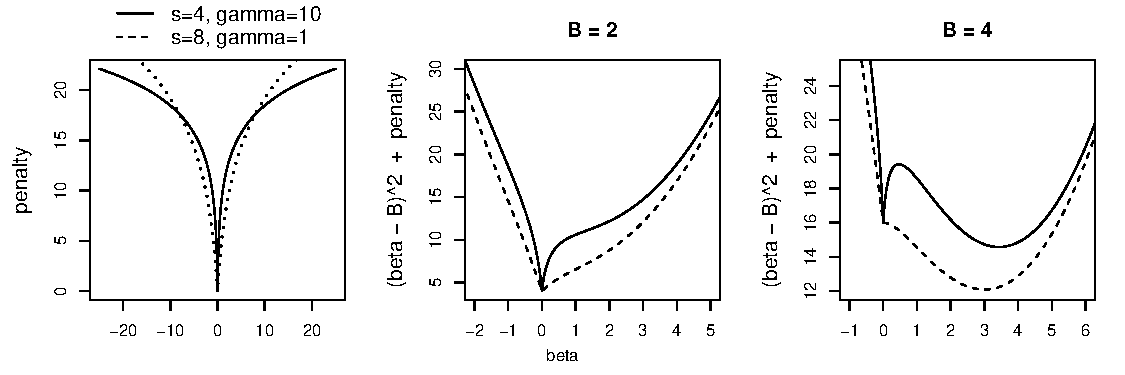
\includegraphics[width=4in]{../graphs/solution}

\vskip .25cm
The solution can jump away from the origin.

\vskip .25cm
This increases estimator variance, and computation cost.
\end{frame}


\begin{frame}
{the gamma lasso}

Each step is just weighted $L_1$ penalized minimization.

\vskip .2cm
Initialize $\bs{\omega}^1 = \bf{1}$ and $\lambda^1 >
0$ with step size
$0 < \delta < 1$.

For $t=1\ldots T:$ 
\vspace{-.25cm}
\begin{align*}
\bs{\hat\beta}^t &= \mr{argmin}~
l(\bs{\beta}) + n\sum \lambda^t\omega^t_j|\beta_j| \\
{\theme \omega^{t+1}_j  }&{\theme = \left(1 + \gamma |\hat\beta^t_j|\right)^{-1}}, ~~j=1\ldots p,~~ \lambda^{t+1} = \delta \lambda^t
\end{align*}

We get diminishing bias since $\omega^{t+1}_j$ decreases with $\gamma |\hat\beta^t_j|$.

\vskip .2cm
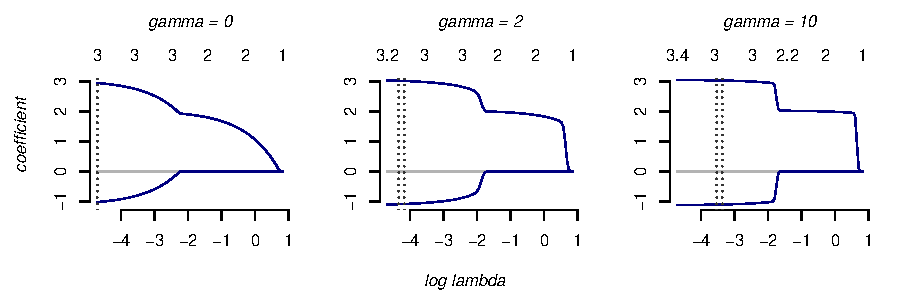
\includegraphics[width=4.1in]{../graphs/gamlr_eg}
\vskip -1cm
\end{frame}


\begin{frame}
{GL as a heuristic}

{\theme Bayes:} under Laplace-gamma prior 
\[
\mr{La}\left(\beta ; \tau\right)\mr{Ga}\left(\tau; s,\gamma^{-1}\right)
\]
the conditional MAP is $\hat\tau | \beta = \gamma s/(1 + \gamma |\beta|)$.  

\vskip .2cm Writing $s = n\lambda/\gamma$, GL plugs this in for $\hat\tau^t_j$ given $\hat \beta^t_{j-1}$.



\vskip .35cm 
{\theme Log penalty:} true joint MAP of this prior implies $s\log(1+\gamma|\beta|)$ costs; that's what GL approaches as $\lambda_t\rightarrow \lambda_{t+1}$.

\end{frame}

\begin{frame}
{diminishing bias via weighted $L_1$ penalization}

The {\nv Adaptive lasso} (Zou) uses pre-estimates (e.g., OLS, marginal, other lasso) of $\bs{\beta}$ as inverse weights on $L_1$ cost.\\
{\gr Basically same as a step of GL, which I call `path adaptation'.}

\vskip .25cm 
Anything fit by {\nv local linear approximation} (LLA; e.g., Candes et al, Fan et al) is iterating through many weighted lassos.  

\vskip .25cm
Authors inspired by Bickle's {\nv one-step estimation} (OSE)  show that stopping LLA after 1-2 steps is as good (or better) than waiting for convergence {\small (e.g., Zou{\tt +}Li 08, Fan, Xue, Zou 2014).}  

\vskip .25cm
OSE depends on starting close enough to best that a single iteration is  statistically optimal.  Path algorithms rely on $\bs{\hat\beta}_t$ being a good hot start for $\bs{\hat\beta}_t$.  {\theme They are natural partners!}

\end{frame}

\begin{frame}
{weighted lasso properties}

How do weighted lassos compare to the \\most concave penalty possible: {\theme $L_0$ cost?}

\vskip .5cm
{\it Definitions}

\vskip .25cm
For $S \subset 1\ldots p$ with $|S|=s$, denote vectors
restricted \\to $S$ as $\bm{\beta}_S = [\beta_j:j\in S]'$, matrices  as $\bm{X}_S$, etc.  

\vskip .25cm $\bs{\beta}^S$ denotes OLS restricted to $S$: \\
~~~~~~~~~~$\bs{\beta}^S_S = (\bm{X}_S'\bm{X}_S)^{-1}\bm{X}_S'\bm{y}$ and $\beta^{S}_j = 0~\forall~j\notin S$

\vskip .25cm
A restricted eigenvalue (RE) is
\vspace{-.25cm}\[
\phi^2(L,S) = \min_{\{\bm{v}: \bm{v}\neq \bm{0},~|\bm{v}_{S^c}| \leq L\sqrt{s}\|\bm{v}_S\|\}}\frac{\|\bm{X}\bm{v}\|^2}{n\|\bm{v}\|^2}.
\]

\end{frame}

\begin{frame}
{sparse approximation}

Consider squared-error loss $l(\bs{\beta}) =
\frac{1}{2}\|\bm{X}\bs{\beta}-\bm{y}\|^2$.

\vskip .25cm
Suppose $\bs{\beta}^{\nu}$ minimizes the $L_0$ penalized objective $l(\bs{\beta}) + n\nu\sum_{j=1}^p\ds{1}_{\{\beta_j\neq0\}}$ with $\bs{\beta}^\nu = \bs{\beta}^S$ and $|S|=s<n$. 

\vskip .25cm   
Write $\bs{\hat\beta}$ as solution to minimize $l(\bs{\beta}) + n\lambda\bs{\omega}'|\bs{\beta}|$. 

\vskip .25cm   
{\theme Theorem:} 
$\omega^{\mr{min}}_{S^c}\lambda > \sqrt{2\nu}$ while $\phi^2(L,S) > 0$ implies
\begin{equation*} \frac{\|\bm{X}(\bs{\hat\beta}-\bs{\beta}^\nu)\|^2}{n}\leq
\frac{4\lambda^2 \|\bs{\omega}_S\|^2}{\phi^2(L, S)}
\end{equation*} 
with 
 $L = \frac{\|\bs{\omega}_S\|}{\sqrt{s}}(\omega^{\mr{min}}_{S^c}-\sqrt{2\nu}/\lambda)^{-1}$.
\end{frame}

\begin{frame}
{optimal sparse approximation}

Recall that GL weights will decrease faster with big $\gamma$.

\sk
Suppose that $\bm{y} \sim
(\bm{f},\sigma^2\bm{I})$.

\vskip .25cm
Mallows' $C_p$ suggests choosing $S$ to minimize
$\mr{MSE}_S + 2s\sigma^2/n$. 

\vskip .25cm Implies $\nu = \sigma^2/n$ and $L = \frac{\|\bs{\omega}_S\|}{\sqrt{s}}\left(\omega^{\mr{min}}_{S^c}- \sqrt{2}\sigma/(\lambda/\sqrt{n})\right)^{-1}$.

\vskip .25cm
Condition on min weight is then
$\omega^{\mr{min}}_{S^c} > (\sigma/\lambda)\sqrt{2/n}$, \\so $C_p$ suggests we  can use larger $\gamma$ with large $n$ or small $\sigma$.
\end{frame}

\begin{frame}
{sign recovery}

A massive amount of effort (too much?) has gone into showing support and sign recovery for concave penalized estimators.

\vskip .25cm
You get $L_0$ estimator sign recovery from weighted $L_1$ estimation, but only under a weighted irrepresentable condition (ii below).

\vskip .25cm
{\theme Theorem:} Under same setting as above, $\mr{sgn}(\bs{\hat\beta}) = \mr{sgn}(\bs{\beta}^\nu)$ if

\vskip .2cm
$\displaystyle ~~~~~~\mr{(i)}~~~\frac{1}{n}\bs{x}_j'\bm{y} > \lambda\omega_j ~~\forall~j \in S$

\vskip .2cm
$\displaystyle ~~~~~~\mr{(ii)}~~~|\bs{x}_j'\bm{X}_S(\bm{X}_S'\bm{X}_S)^{-1}\bs{\omega}_S| \leq 1 - \frac{\sqrt{2\nu}}{\lambda\omega_j} ~~\forall~j \in S^c.
$

\vskip .25cm
{\gr Things are more pessimistic without (ii), \\unless you can make $\omega_j$ very big for $j\in S^c$.}

\end{frame}

\begin{frame}
{Concavity and Stability }

Recall: $\omega^{t+1}_j = 1/\left(1 + \gamma |\hat\beta^t_j|\right)$

\vskip .25cm
The $\gamma$ parameter governs how quickly bias disappears:\\
\hfill $\gamma=0$ is the lasso, and $\gamma = \infty$ is subset selection.

\vskip .25cm
{What are we giving away?  How stable is the procedure?}

\vskip .5cm
GL has a nice type of theoretical stability for all $\gamma < \infty$:\\ \hfill  Lipschitz continuity with respect to jitter in the response $\bm{y}$.

\vskip .15cm
{\gr $f$ is Lipschitz continuous if  $ |f(b_1)-f(b_2)| \leq
L|b_1-b_2| $ \\for some finite constant $L$ on all $b_1,b_2$ in the domain of
$f$.} 

\vskip .15cm
Intuitively, this requires Lipschitz regularization paths.

\vskip .25cm
{\nv Sub-optimality of the one-step-estimator gives us this stability.}

\end{frame}


\begin{frame}

Be careful: Lipschitz does not guarantee `practical' stability.

\vskip .25cm
e.g., Making $\gamma$ too big causes timings to blow up.
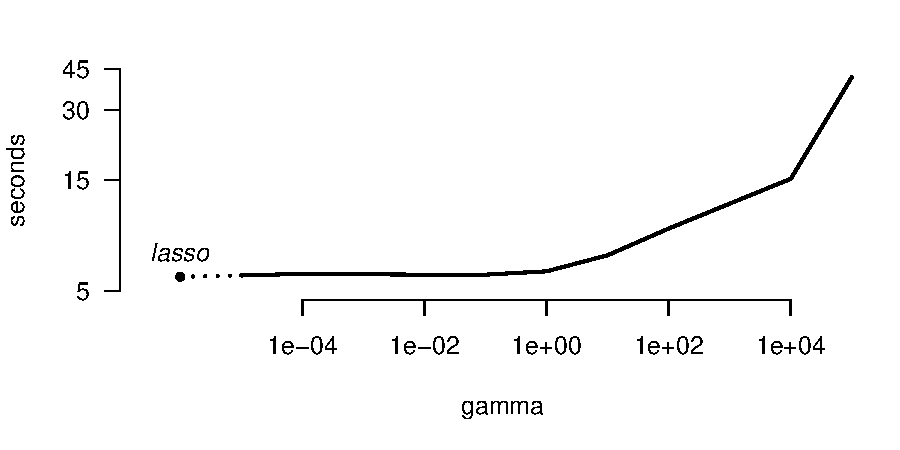
\includegraphics[width=4in]{../graphs/nhl_time}

This is because $\bs{\hat\beta}^{t-1}$ become bad hot-starts 
for $\bs{\hat\beta}^t$.

\end{frame}

\begin{frame}

{\bf  $\lambda$ just indexes models.  \theme How do you choose?}

\vskip .2cm
~~~~~~~~~~~e.g., AICc = deviance($\bs{\hat\beta}$) + 2$df\frac{n}{n-df-1}$.

\vskip .5cm
Useful benefit of Lipschitz: use Stein's $df = \ds{E}\left[\sum_i \partial \hat
y_i/\partial y_i\right]$.

\vskip .25cm
Zou et al. 2007 apply this with lasso ($L1$) penalties
\[
\ds{E}\left[ \ds{1}_{[|g_j|<\tau_j]} \right] \approx \sum_j |g_j| < \omega_j\lambda 
\]
\vskip -.35cm
where $g_j$ is $\partial l /\partial x_j |_{\hat \beta_j=0}$.

\vskip .5cm
Use the Bayesian model to get heuristic version for GL:
\[\nv
\widehat{df} = \sum_j \pi(|g_j| < \omega_j\lambda) \gr = \sum_j \mr{Ga}(|g_{j}|;~ n\lambda/\gamma, 1/\gamma).
\]
\vskip -1cm

\end{frame}

\begin{frame}

{\bf An example: \theme NHL hockey players}

\vskip .25cm
Every goal back to 2002-2003:
64540 goals and 2302 players.

\vskip .25cm
Our `regression plus-minus' model {\gr({\small Gramacy, Jensen, Taddy})}:
\[
\mr{logit}\left[\mr{p}(\text{home~team~scored~goal}~i)\right] = \alpha +
\bm{u}'\bs{\varphi} + \bm{x}'\bs{\beta}, 
\]


$x_{ij}=1$ if player $j$ was on the home team and on ice for goal $i$, $x_{ij}=-1$ for away player
$j$ on ice, and $x_{ij}=0$ otherwise.  

\vskip .1cm 
$\bm{u}$ includes controls: team$\times$season, special-teams scenarios.

\vskip .25cm {\nv $\Rightarrow \beta_j$ is the  effect of a player on the log odds
that, given a goal has been scored, the goal was scored by his team.}

\vskip .25cm
We'll fit a GL path  for $\bs{\beta}$, leave $\bs{\varphi}$ unpenalized.

\end{frame}

\begin{frame}

{\bf \theme Hockey GL paths}

\vskip .5cm
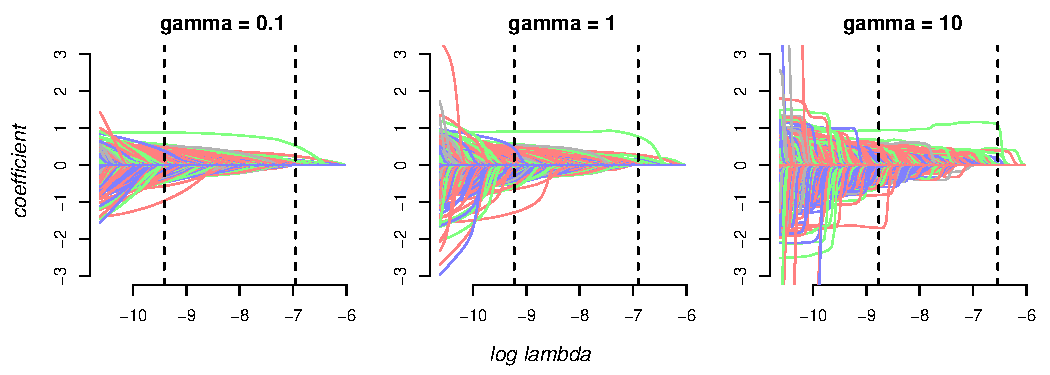
\includegraphics[width=4.25in]{../graphs/nhl_paths}

\sk
Minimum AIC and BIC are marked with the  vertical lines.

\vskip .1cm
grey:goalie, blue:defense, green:center, red:winger.

\end{frame}

\begin{frame}


{\bf \theme Hockey IC surfaces}

\vskip .5cm
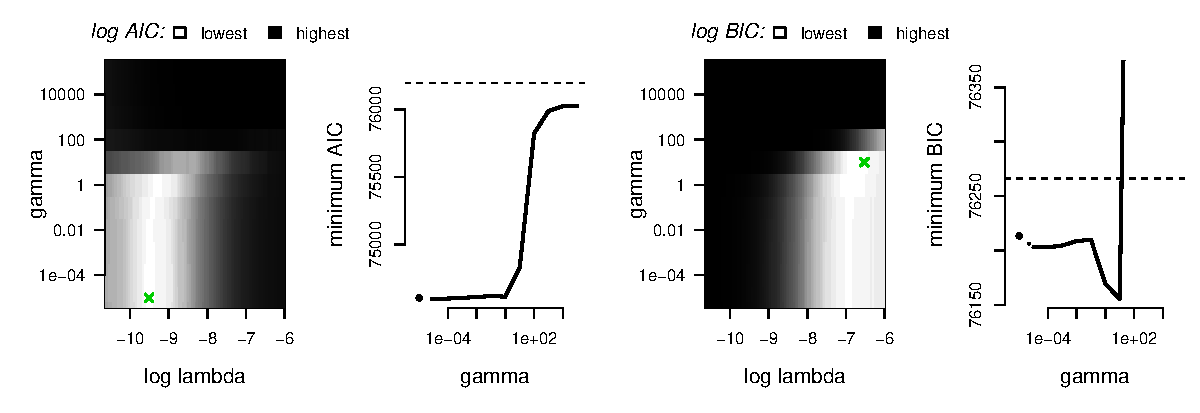
\includegraphics[width=4.25in]{../graphs/nhl_ic}

\vskip .5cm
AIC favors dense high-shrinkage models, \\BIC likes sparse low-shrinkage.

\vskip .25cm
Both seem to hate [practical] instability.
\end{frame}

\begin{frame}

{\bf \theme Hockey 20-fold CV}

\sk
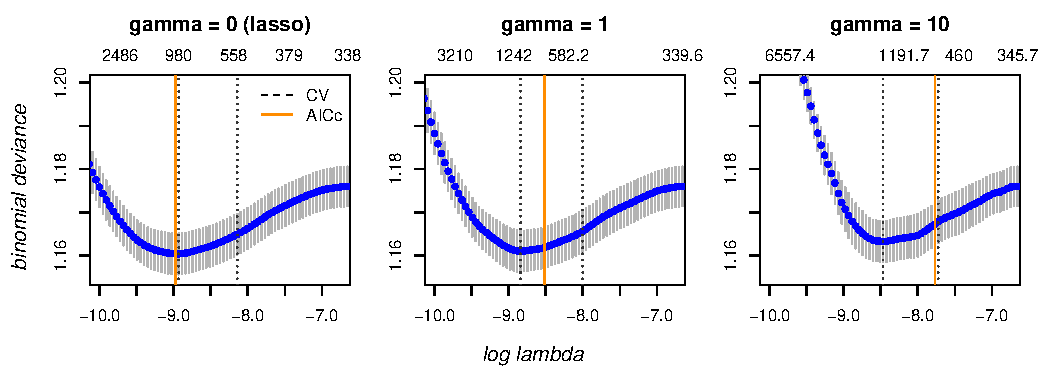
\includegraphics[width=4.25in]{../graphs/nhl_cv}

\sk
Some predictive benefit from small $\gamma>0$.
\vskip .2cm
For larger $\gamma$, you just get more variability.

\vskip .25cm
But increasing $\gamma$ does change our story about contributions.

\end{frame}

\begin{frame}
{partial plus minus}

First, convert from player $\beta_j$ to the scale of `plus/minus'.

\vskip .25cm
If we know nothing else (not team, home/away, etc), then the probability a goal was scored by his team given player $j$ is on ice becomes
$p_j = e^{\beta_j}/(1+e^{\beta_j})$ and our `partial plus/minus' is
\[
\mr{ppm}_j = N_j(p_j - (1-p_j)) = N_j(2p_j-1)
\]
where $N_j$ is the total \# of goals he was on-ice for.

\vskip .25cm  This measures quality and quantity of contribution.
\end{frame}

\begin{frame}[fragile]{top ten list}

All sorts at AICc for $\gamma=0$ (lasso)

\begin{semiverbatim}\nv\setstretch{1}
 gamma=0: 619 nonzero player effects.
                 player  beta    ppm  pm
 1         ONDREJ_PALAT 0.599 37.257  14
 2        SIDNEY_CROSBY 0.371 28.994  -4
 3       JONATHAN_TOEWS 0.287 22.908   5
 4        ANDREI_MARKOV 0.261 22.612  -6
 5     HENRIK_LUNDQVIST 0.132 21.742  49
 6         JOE_THORNTON 0.363 20.841 -22
 7         ANZE_KOPITAR 0.221 19.930  29
 8  RYAN_NUGENT-HOPKINS 0.270 17.994   2
 9        PAVEL_DATSYUK 0.363 17.778 -13
 10   GABRIEL_LANDESKOG 0.239 16.868  26
\end{semiverbatim}


\end{frame}


\begin{frame}[fragile]{top ten list}

$\gamma=1$ brings up Sid to \#1 and introduces Toffoli.

\begin{semiverbatim}\nv\setstretch{1}
  gamma=1: 591 nonzero career effects
                 player  beta    ppm  pm
 1        SIDNEY_CROSBY 0.402 31.353  -4
 2        TYLER_TOFFOLI 0.825 29.288  11
 3         ONDREJ_PALAT 0.419 26.425  14
 4       JONATHAN_TOEWS 0.314 25.063   5
 5        ANDREI_MARKOV 0.276 23.819  -6
 6     HENRIK_LUNDQVIST 0.137 22.719  49
 7         ANZE_KOPITAR 0.246 22.162  29
 8         JOE_THORNTON 0.376 21.534 -22
 9  RYAN_NUGENT-HOPKINS 0.318 21.137   2
 10   GABRIEL_LANDESKOG 0.278 19.599  26
\end{semiverbatim}

\end{frame}


\begin{frame}[fragile]{top ten list}

$\gamma=10$ leaves only big name big minute guys.

\begin{semiverbatim}\nv\setstretch{1}
 gamma=10: 136 nonzero player effects
             player  beta    ppm  pm
 1    SIDNEY_CROSBY 0.411 32.055  -4
 2     ANZE_KOPITAR 0.245 22.102  29
 3     JOE_THORNTON 0.385 22.037 -22
 4   JONATHAN_TOEWS 0.269 21.540   5
 5    ANDREI_MARKOV 0.240 20.769  -6
 6    LOGAN_COUTURE 0.421 20.133 -27
 7    ALEX_OVECHKIN 0.355 19.299 -14
 8    JORDAN_EBERLE 0.291 18.084   9
 9    PAVEL_DATSYUK 0.340 16.672 -13
 10 ALEXANDER_SEMIN 0.376 16.157  17
\end{semiverbatim}

\end{frame}

\begin{frame}

\begin{center}
\Huge \theme Thanks!
\end{center}

\vskip 1cm
Papers at {\tt faculty.chicagobooth.edu/matt.taddy/research} \\{\gr(revised GL draft soon)}

\vskip .25cm hockey data and code at {\tt github.com/mataddy/hockey}.

\vskip .25cm and R package {\tt gamlr} for all your weighted lasso needs.

\end{frame}

\end{document}
